\mode
<article>

%% Markup
\markdownSetupSnippet{horizontalRule/singleFrame}{snippet=witiko/beamer/MU/horizontalRule/singleFrame}

%% Title page
\maketitle

\mode
<presentation>

%% Markup
\markdownSetupSnippet{horizontalRule/frameBreak}{snippet=witiko/beamer/MU/horizontalRule/frameBreak}
\markdownSetupSnippet{headingTwo/several}{snippet=witiko/beamer/MU/headingTwo/several}

%% Title page
\begin{frame}[plain]
\begin{tikzpicture}[overlay, remember picture]
  \node[anchor=south east, xshift=254.5pt, yshift=-27pt] at (current page.south east) {
    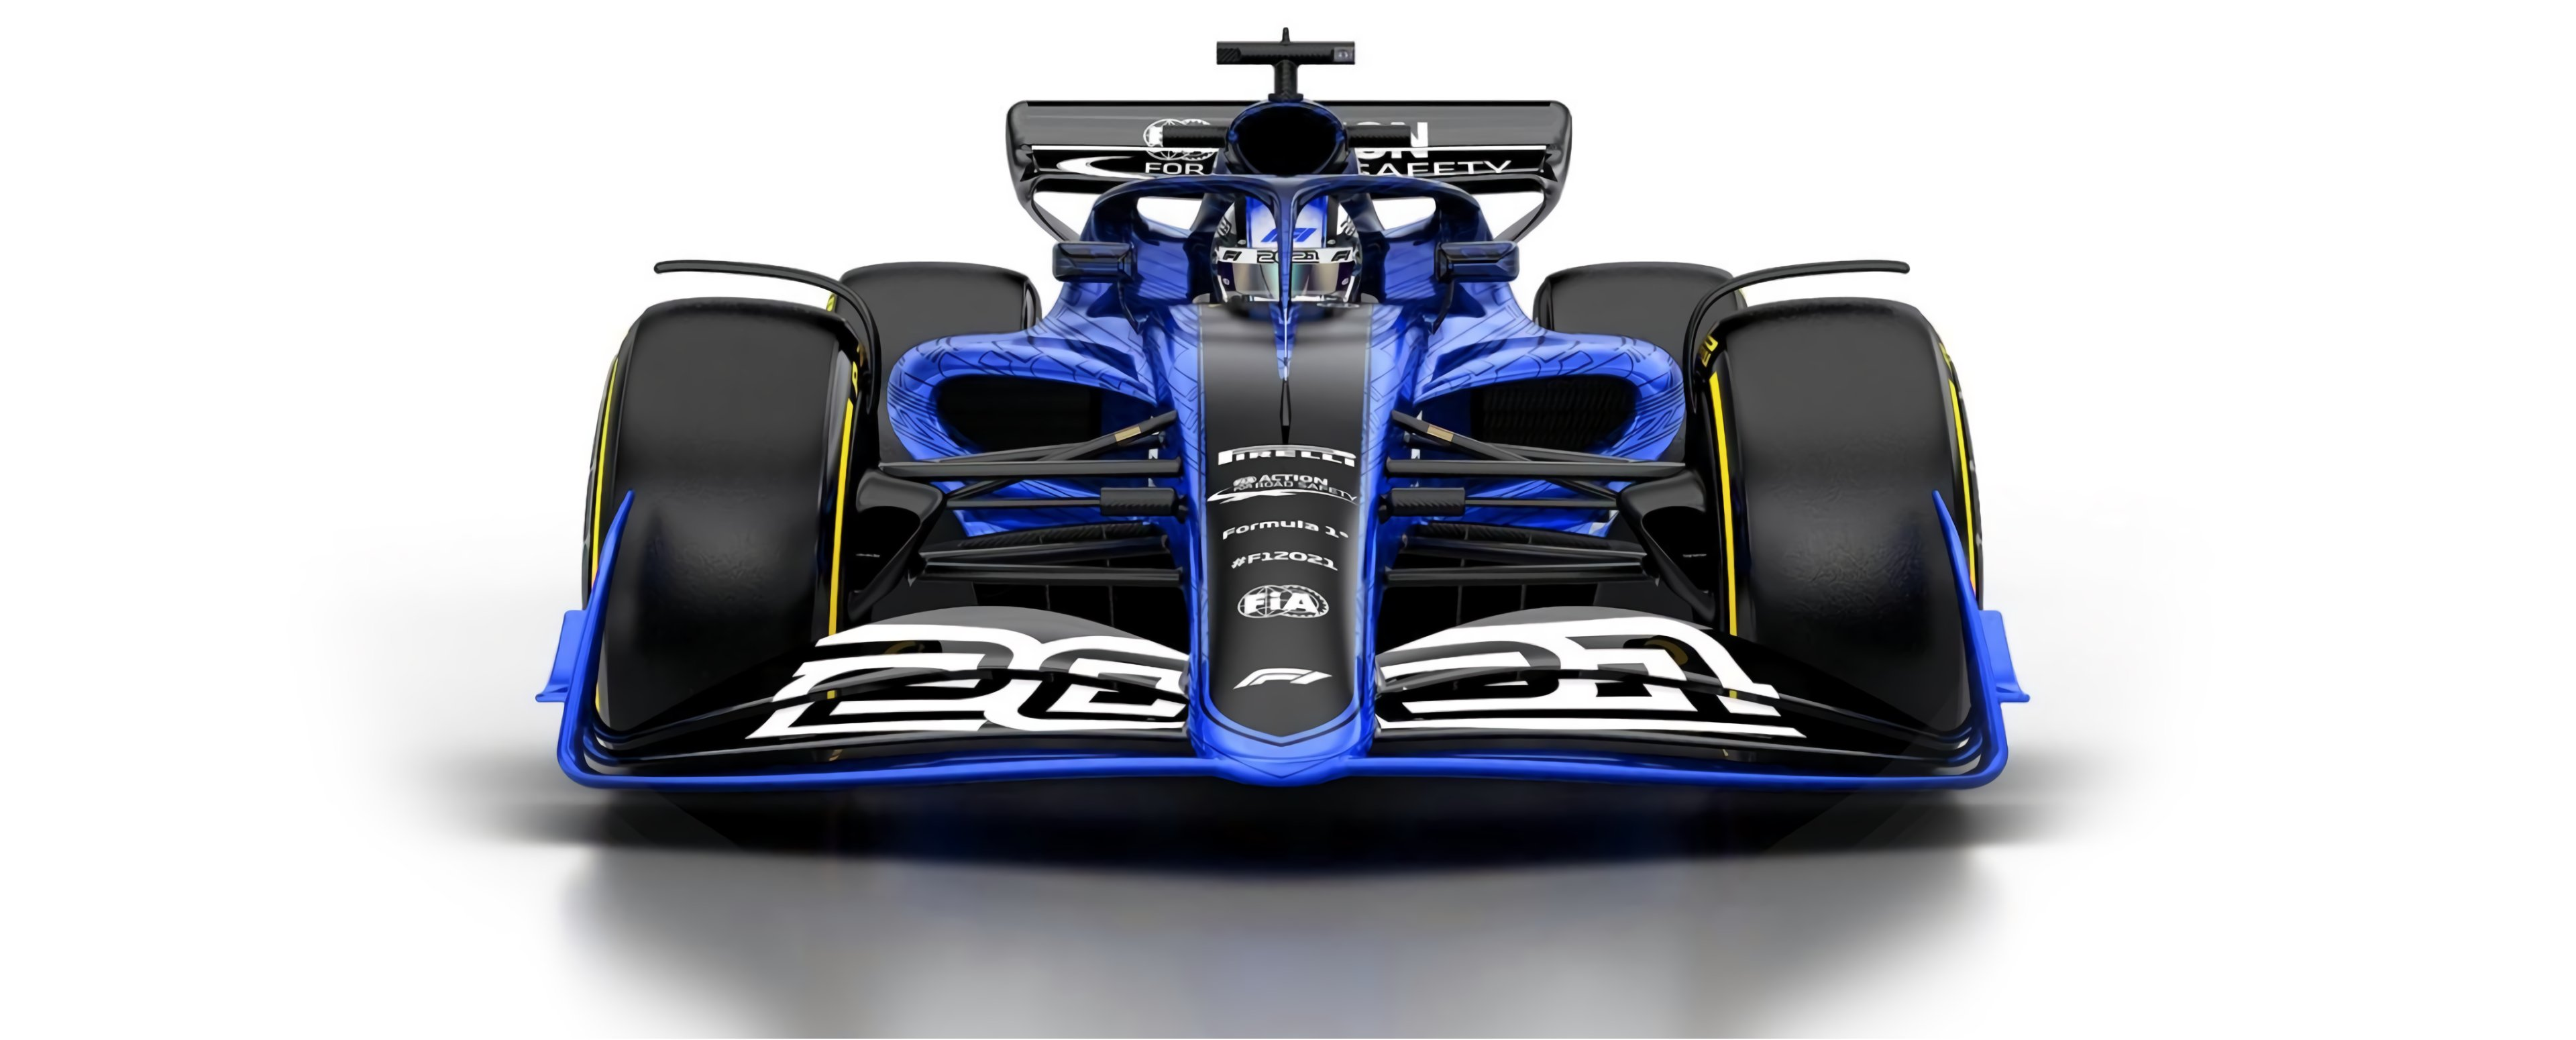
\includegraphics[height=0.91\textheight]{formula1}
  };
\end{tikzpicture}
\maketitle
\end{frame}

%% Graphics
\setkeys{Gin}{
  width = \columnwidth,
  height = \paperheight,
  keepaspectratio,
}

\mode
<article>

\part{Summary}

% Introduction
\markdownInput[slice=^ ^introduction]{defense.md}
\markdownInput[slice=introduction ^research-questions]{defense.md}
\markdownInput[slice=research-questions, snippet=horizontalRule/singleFrame]{defense.md}
\markdownInput[slice=thesis-structure]{defense.md}

% Background
\markdownInput[slice=digital-mathematical-libraries]{defense.md}
\markdownInput[slice=math-representations]{defense.md}
\markdownInput[slice=math-information-retrieval]{defense.md}
\markdownInput[slice=objectives-and-evaluation]{defense.md}

% State of the Art
\markdownInput[slice=competitions]{defense.md}
\markdownInput[slice=systems]{defense.md}

% Accuracy and Speed
\markdownInput[slice=accuracy-and-speed ^representations,
               snippet=horizontalRule/singleFrame]{defense.md}
\markdownInput[slice=representations]{defense.md}
\markdownInput[slice=learning-to-rank]{defense.md}
\markdownInput[slice=approximate-search]{defense.md}

% Interpretability
\markdownInput[slice=interpretability ^interpretable-representations,
               snippet=horizontalRule/singleFrame]{defense.md}
\markdownInput[slice=interpretable-representations]{defense.md}
\markdownInput[slice=strengths-and-weaknesses]{defense.md}
\markdownInput[slice=interactive-visualizations]{defense.md}

% Conclusion
\markdownInput[slice=conclusion]{defense.md}

% List of Author's Publications
\markdownInput[slice=list-of-publications]{defense.md}

\part{Rebuttal}

\markdownInput[slice=common-remarks]{defense.md}

\markdownInput[slice=oard ^soft-cosine-measure-questions,
               snippet=horizontalRule/singleFrame]{defense.md}
\markdownInput[slice=soft-cosine-measure-questions]{defense.md}
\markdownInput[slice=sentence-bert-questions]{defense.md}
\markdownInput[slice=system-combination-questions]{defense.md}
\markdownInput[slice=interpretable-representation-questions]{defense.md}

\markdownInput[slice=skopal ^defense-questions,
               snippet=horizontalRule/singleFrame]{defense.md}
\markdownInput[slice=defense-questions]{defense.md}

\printbibliography

\mode
<presentation>

\part{Summary}
\frame{\vfill\partpage\vfill}

\section{Introduction}
\begin{frame}[fragile]
  \markdownInput[slice=introduction ^research-questions]{defense.md}
\end{frame}

\subsection{Research Questions}
\begin{frame}[fragile]{\secname}
  \markdownInput[slice=research-questions]{defense.md}
  \markdownInput[slice=thesis-structure,
                 snippet=headingTwo/several]{defense.md}
\end{frame}

\section{Background}
\subsection{Digital Mathematical Libraries}
\begingroup
\setbeamertemplate{footline}{}
\begin{frame}[fragile, allowframebreaks=1.2]{\secname}
  \markdownInput[slice=digital-mathematical-libraries,
                 snippet=horizontalRule/frameBreak]{defense.md}
\end{frame}
\endgroup

\subsection{Math Representations}
\begingroup
\setbeamertemplate{footline}{}
\begin{frame}[fragile]{\secname}
  \markdownInput[slice=math-representations]{defense.md}
\end{frame}
\endgroup

\subsection{Math Information Retrieval}
\begingroup
\setbeamertemplate{footline}{}
\begin{frame}[fragile, allowframebreaks=1.2]{\secname}
  \markdownInput[slice=math-information-retrieval,
                 snippet=horizontalRule/frameBreak]{defense.md}
\end{frame}
\endgroup

\subsection{Objectives and Evaluation}
\begin{frame}[fragile]{\secname}
  \markdownOlColumns=3
  \markdownInput[slice=objectives-and-evaluation]{defense.md}
\end{frame}

\section{State of the Art}
\subsection{Competitions}
\begin{frame}[fragile]{\secname}
  \markdownInput[slice=competitions]{defense.md}
\end{frame}

\subsection{Systems}
\begin{frame}[fragile]{\secname}
  \markdownInput[slice=systems]{defense.md}
\end{frame}

\section{Accuracy and Speed}

\subsection{Math Representations and Representation Learning}
\begin{frame}[fragile, allowframebreaks=1.2]{\secname}
  \markdownInput[slice=representations,
                 snippet=horizontalRule/frameBreak]{defense.md}
\end{frame}

\subsection{Learning to Rank}
\begin{frame}[fragile, allowframebreaks=1.2]{\secname}
  \markdownInput[slice=learning-to-rank,
                 snippet=horizontalRule/frameBreak]{defense.md}
\end{frame}

\subsection{Approximate Nearest-Neigbor Search}
\begin{frame}[fragile, allowframebreaks=1.2]{\secname}
  \markdownInput[slice=approximate-search,
                 snippet=horizontalRule/frameBreak]{defense.md}
\end{frame}

\section{Interpretability}

\subsection{Representation Learning of Words and Symbols}
\begin{frame}[fragile, allowframebreaks=1.2]{\secname}
  \markdownInput[slice=interpretable-representations,
                 snippet=horizontalRule/frameBreak]{defense.md}
\end{frame}

\subsection{Strengths and Weaknesses of Retrieval Systems}
\begin{frame}[fragile]{\secname}
  \markdownInput[slice=strengths-and-weaknesses]{defense.md}
\end{frame}

\subsection{Interactive Visualizations of Retrieval Collections}
\begingroup
\usebackgroundtemplate{%
  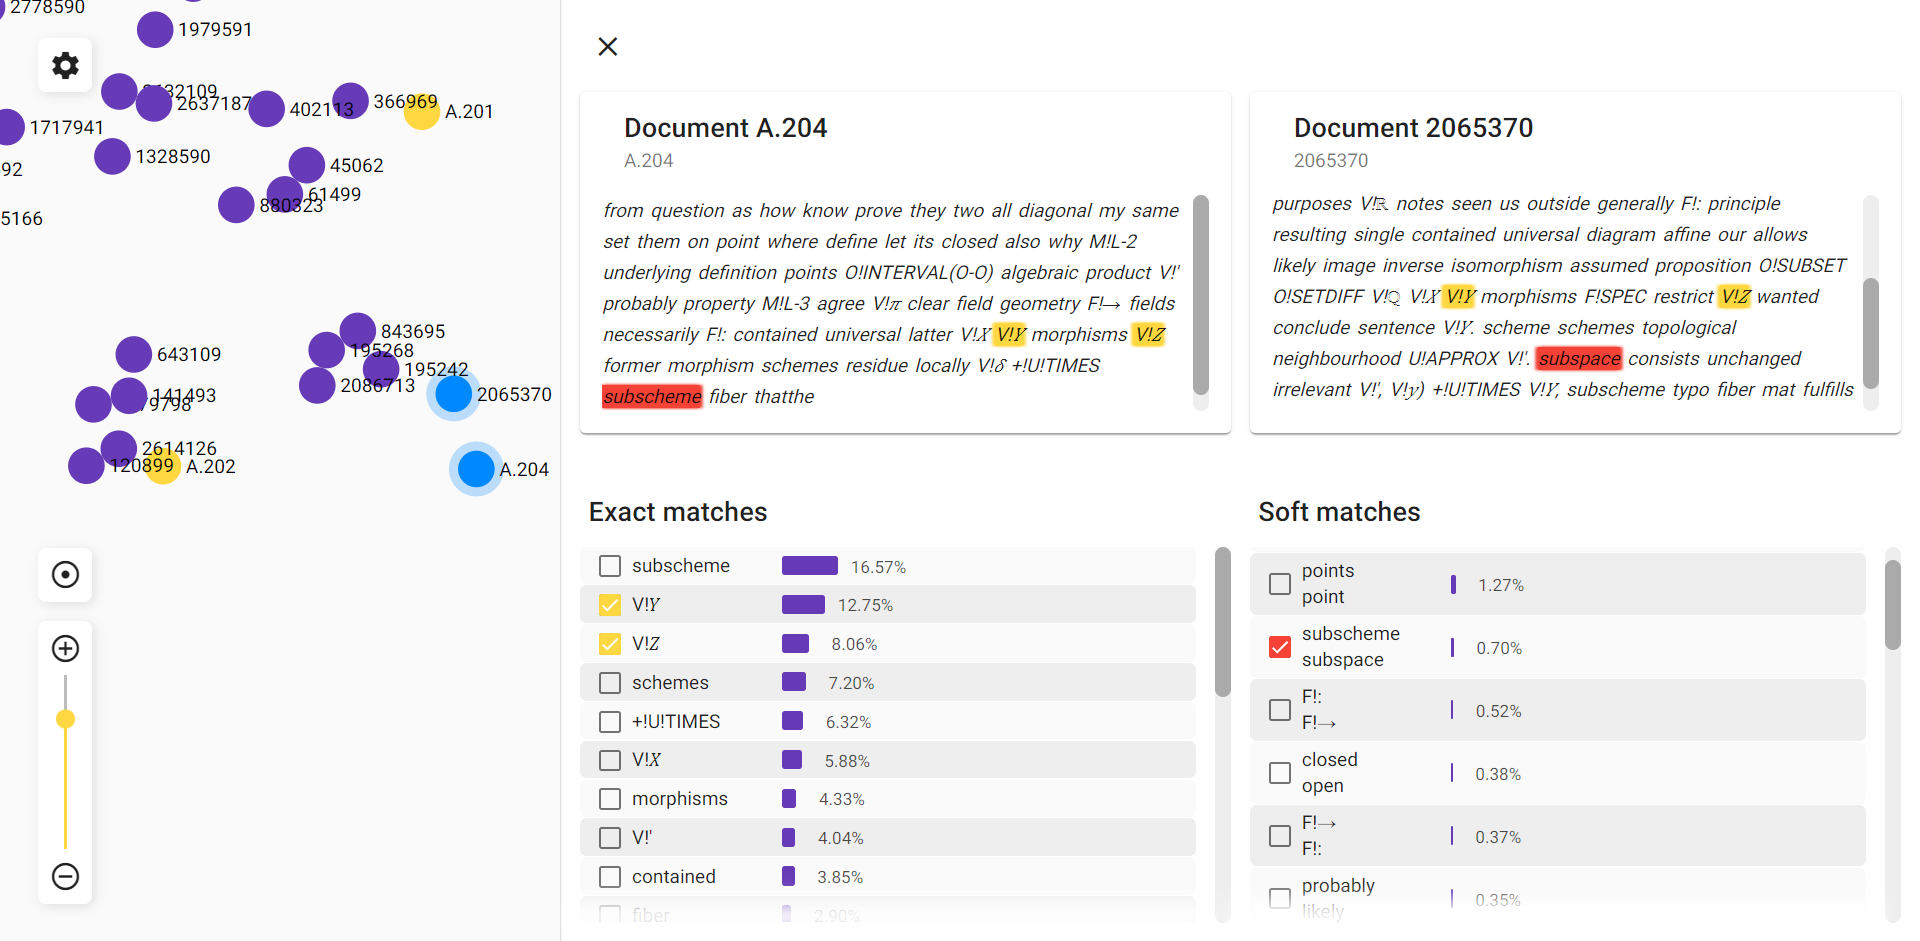
\includegraphics[width=\paperwidth, height=\paperheight]{document-maps}%
}
\begin{frame}[fragile, plain]
\end{frame}
\endgroup

\section{Conclusion}
\begin{frame}[fragile]
  \markdownInput[slice=conclusion]{defense.md}
\end{frame}

\section{List of Author's Publications}
\begin{frame}[fragile]
  \markdownInput[slice=list-of-publications]{defense.md}
\end{frame}

\begin{frame}[plain]
\vfill\vfill
\centerline{Thank You for Your Attention!}
\vfill\vfill\vfill
\end{frame}

\part{Rebuttal}
\frame{\vfill\partpage\vfill}

\section{Common Remarks}

\begin{frame}[fragile]{\secname}
  \markdownInput[slice=common-remarks]{defense.md}
\end{frame}

\section{Response to the report of prof.\ Douglas W.\ Oard}

\subsection{Soft Cosine Measure Questions}
\begin{frame}[fragile, allowframebreaks=1.2]{\secname}
  \markdownInput[slice=soft-cosine-measure-questions,
                 snippet=horizontalRule/frameBreak]{defense.md}
\end{frame}

\subsection{Sentence-BERT Questions}
\begin{frame}[fragile, allowframebreaks=1.2]{\secname}
  \markdownInput[slice=sentence-bert-questions,
                 snippet=horizontalRule/frameBreak]{defense.md}
\end{frame}

\subsection{System Combination Questions}
\begin{frame}[fragile]{\secname}
  \markdownInput[slice=system-combination-questions]{defense.md}
\end{frame}

\subsection{Interpretable Representation Questions}
\begin{frame}[fragile, allowframebreaks=1.2]{\secname}
  \markdownInput[slice=interpretable-representation-questions,
                 snippet=horizontalRule/frameBreak]{defense.md}
\end{frame}

\section{Response to the report of prof.\ RNDr.\ Tomáš Skopal, Ph.D.}

\subsection{Defense Questions}
\begin{frame}[fragile, allowframebreaks=1.2]{\secname}
  \markdownInput[slice=defense-questions,
                 snippet=horizontalRule/frameBreak]{defense.md}
\end{frame}

\begin{frame}[plain]
\vfill\vfill
\centerline{Thank You for Your Attention!}
\vfill\vfill\vfill
\end{frame}

\part{\bibname}
\frame{\vfill\partpage\vfill}

\section{\bibname}
\begin{frame}[allowframebreaks]{\bibname}
\printbibliography[heading=none]
\end{frame}

\mode
<all>
